\documentclass[10pt,a4paper]{article}
\usepackage[utf8]{inputenc}
\usepackage[german]{babel}
\usepackage{amsmath}
\usepackage{amsfonts}
\usepackage{amssymb}
\usepackage{setspace}
\usepackage{graphicx} %Um Bilder anzeigen zu können
\usepackage[top=1in, bottom=1.5in, left=1in, right=1in]{geometry}
\usepackage{endnotes}

\let\footnote=\endnote

\title{\Huge Entwurf\\[1cm] {\bfseries Praxis der Softwareentwicklung}\\[2cm] Entwicklung einer Software zur Berechnung der Mandatsverteilung im Deutschen Bundestag\\[1cm]Gruppe 1}
\author{Philipp Löwer, Anton Mehlmann, Manuel Olk, Enes Ördek, \\Simon Schürg, Nick Vlasoff}
\date{}

\begin{document}
\maketitle
\thispagestyle{empty}

\begin{figure}[h]

\centering
		
		
\includegraphics[scale=0.6]{KIT-Logo.png}\\
		\Huge WS 2013 / 14
\end{figure}

\newpage
\begin{onehalfspace}
\tableofcontents
\end{onehalfspace}
\newpage 

\section{Einleitung}



\section{Systemmodell}


\section{Module}


\subsection{GUI}
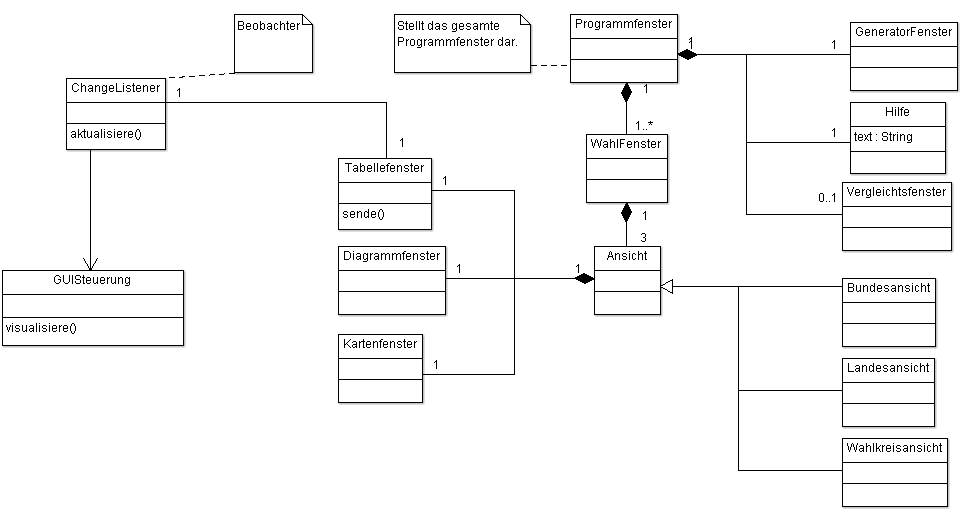
\includegraphics[scale=0.6]{GUI-Abschnitt.png} \\
Dieser Teil des gesamten Klassendiagramms zeigt den Visualisierungsteil. \\
Das Programmfenster besteht aus mehreren Wahlfenstern in Form von Tabs. Weiterhin enthält es
ein Generatorfenster, um nicht identifizierten Parteien Stimmen zu geben, die Hilfe, und
ein Vergleichsfenster, wenn der Vergleich zweier Wahlen aktiv ist. \\
Ein Wahlfenster besteht aus genau drei Ansichtsfenstern, diese sind Bundes-, Landes- und
Wahlkreisansicht.
Zu jeder von diesen gehört jeweils ein Tabellen-, Diagramm- und Kartenfenster. \\
Das Tabellenfenster, in welchem Erst- und Zweitstimmen geändert werden können, und die
dazugehörige ChangeListener-Klasse werden im Beobachter-Prinzip umgesetzt. Der ChangeListener
hört das Tabellenfenster ab und wird bei Veränderungen informiert. \\
Gesteuert werden alle genannten Klassen durch die GUISteuerungs-Klasse, die alle Tabellen befüllt,
Diagramme erstellt und die Kartenfenster füllt. Außerdem werden von ihr auch die Veränderungen,
die der ChangeListener bekommt, verwaltet.

\subsection{Datenhaltung}
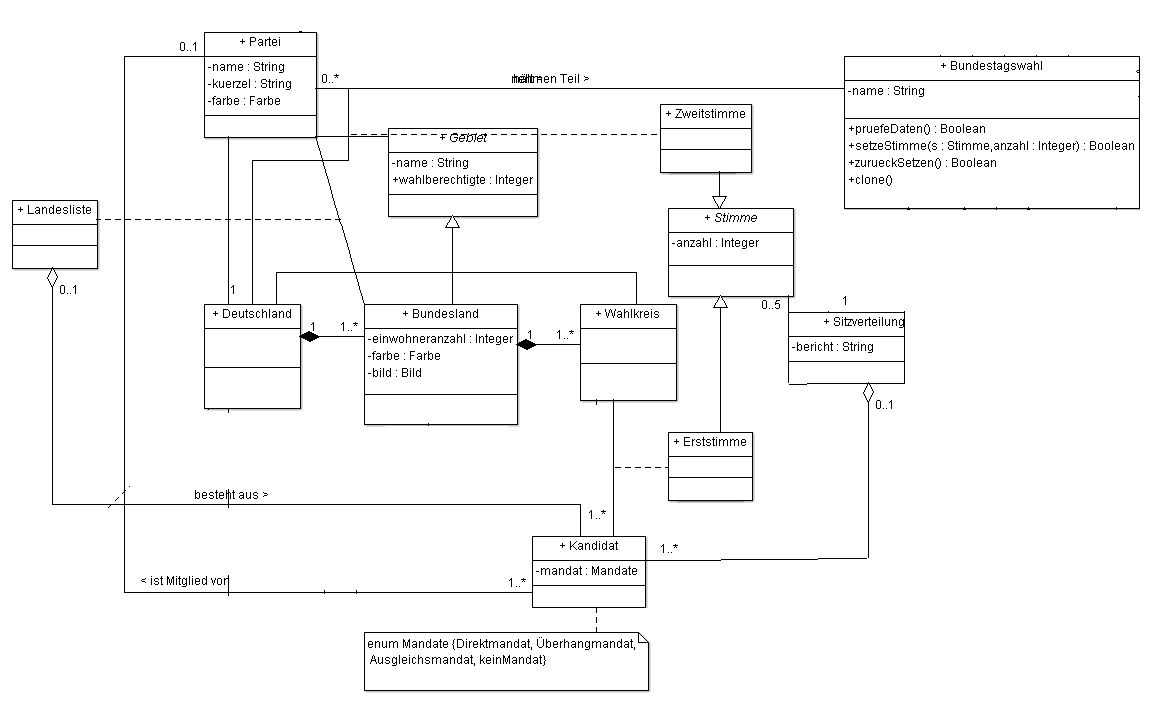
\includegraphics[scale=0.5]{Datenhaltung-Ausschnitt} \\
Dieser Ausschnitt des Klassendiagramms stellt den Datenhaltungsteil dar.

\subsection{Import/ Export}
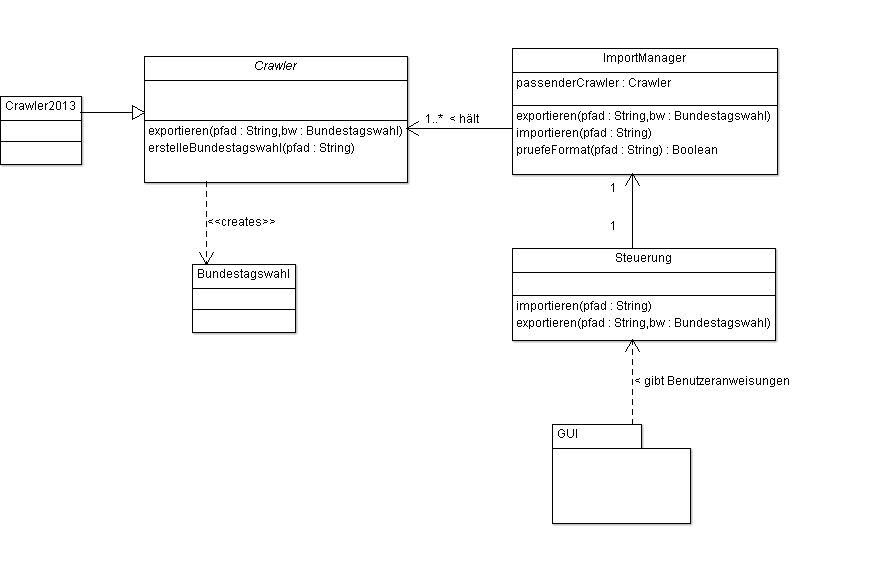
\includegraphics[scale=0.5]{Import-Export Ausschnitt.png} \\
In diesem Klassendiagramm sieht man den Aufbau des Import-/Exportmoduls. Zur Übersichtlichkeit werden die zum Importieren/Exportieren nicht notwendigen Methoden in \textit{Steuerung} und die genaue Struktur hinter \textit{Bundestagswahl} und der GUI ausgeblendet. \\
Mit unserem Programm wird nur ein vorimplementierter Crawler mitgegeben, der .csv-Dateien, die dem Format der .csv-Datei zur Bundestagswahl 2013 der Bundeswahlleiter-Webseite entsprechen, auswerten kann - dies ist \textit{Crawler2013}. Um jedoch die Möglichkeit zu garantieren, nachträglich weitere Crawler hinzuzufügen, haben wir uns dafür entschieden, eine abstrakte Oberklasse \textit{Crawler} zu verwenden, von der \textit{Crawler2013} erbt, und alle vorhandenen Crawler von der Klasse \textit{ImportManager} halten zu lassen. \\ Ausgelöst wird der ganze Import- bzw. Exportvorgang durch eine Benutzerinteraktion (z.B. Betätigen des Laden- Knopfs im Menü), worauf die \textit{GUISteuerung} die \textit{Steuerung} anwählt, welche wiederum über den \textit{ImportManager} den geeigneten Crawler bestimmt, der die Informationen ausliest die eigentliche Arbeit ausführt.

\subparagraph{Methoden}
\begin{description}
\item \textbf {exportieren(pfad : String, bw : Bundestagswahl)} \\
Schreibt die Bundestagswahl bw in die .csv-Datei, deren Pfad in \textbf{pfad} gegeben ist.
\item \textbf {importieren(pfad : String)} \\
Liest die .csv-Datei, deren Pfad in pfad gegeben ist, ein, erstellt ein Bundestagswahlobjekt und füllt es.
\item \textbf{pruefeFormat(pfad : String) : Boolean} \\
Prüft das Format der Datei, deren Pfad in pfad gegeben ist. Wenn es sich um eine .csv-Datei handelt, die durch einen vorhandenen Crawler erfasst werden kann, wird dieser Crawler als passenderCrawler gesetzt und true zurückgegeben. Falls kein geeigneter Crawler gefunden wird, da die Datei keine .csv-Datei ist oder ihre Struktur nicht korrekt ist, wird false zurückgegeben.

\end{description}

\subsection{Wahlgenerierung}
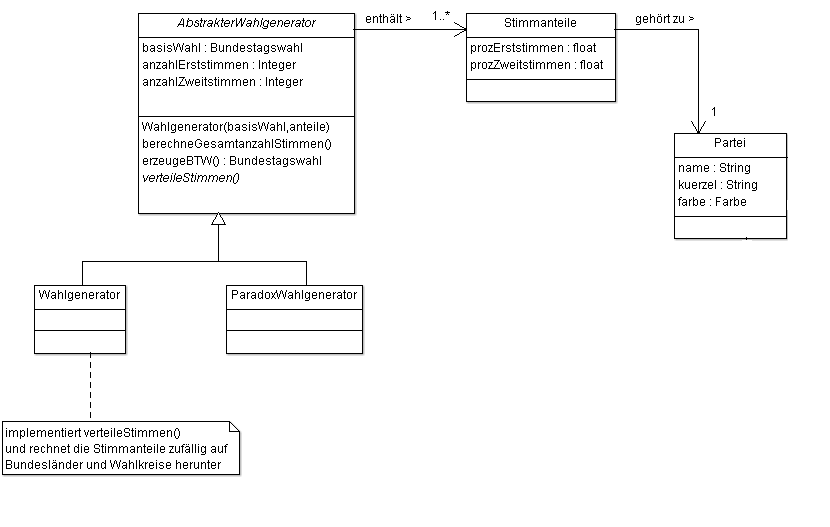
\includegraphics[scale=0.5]{Wahlgenerator_Klassendiagramm.png} \\
Der obige Ausschnitt des Klassendiagramms zeigt das Wahldatengenerierungs-Modul.\\\\
Mit diesem Modul können Bundestagswahlen anhand vorher definierten Stimmanteilen auf Bundesebene generiert werden. Bei diesen Stimmanteilen handelt es sich um eine Liste aller Parteien mit prozentualen Anteilen der Erst- und Zweitstimmen auf Bundesebene. Des weiteren benötigt der Wahlgenerator eine Basis-Bundestagswahl um Daten wie beispielsweise Bundesländer, Wahlkreise und Wahlberechtigte zur Verfügung zu haben.\\\\
Beim generieren einer Bundestagswahl werden die Stimmanteile mithilfe der Anzahl aller Wahlberechtigten in absolute Zahlen für Erst- und Zweitstimmen umgerechnet. Diese Stimmen werden dann zufällig, erst auf alle Bundesländer und dann auf die einzelnen Wahlkreise verteilt.\\\\
Dieser Vorgang ist im folgenden noch einmal als Sequenzdiagramm aufgezeigt.\\\\
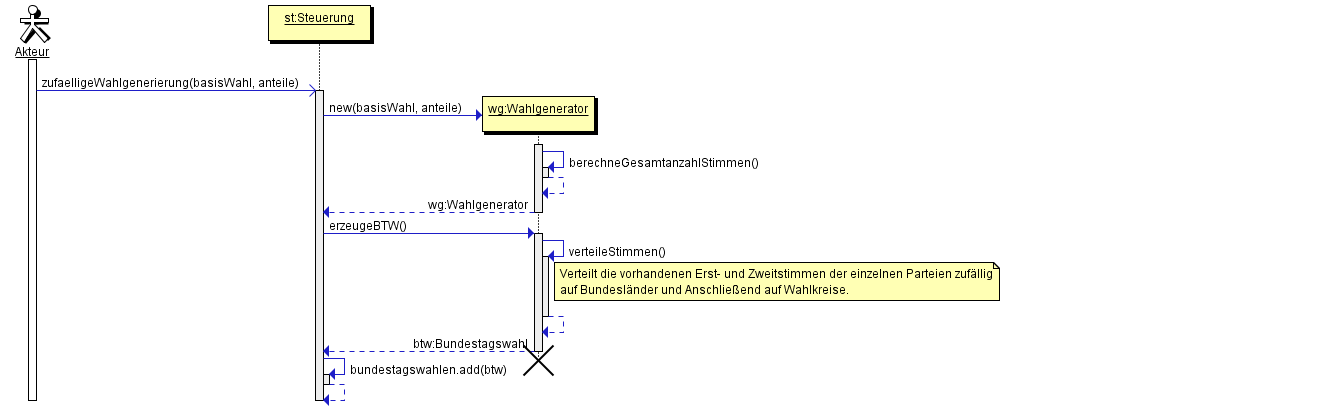
\includegraphics[scale=0.5]{zufaelligeWahlgenerierung_Sequenzdiagramm.png}
Neben der zufälligen Verteilung von den Stimmen auf alle Bundesländer und Wahlkreise gibt es noch einen Wahlgenerator der Stimmverteilungen erzeugt, die nach dem Wahlgesetz von 2009 zu negativem Stimmgewicht durch Überhangsmandate führen. Diese werden benötigt um in einer Vergleichsansicht das negative Stimmgewicht zu verdeutlichen.

\subsection{Chronik}



\section{Anwendungsfälle}



\section{Sequenzdiagramme}
\subsection{Import}
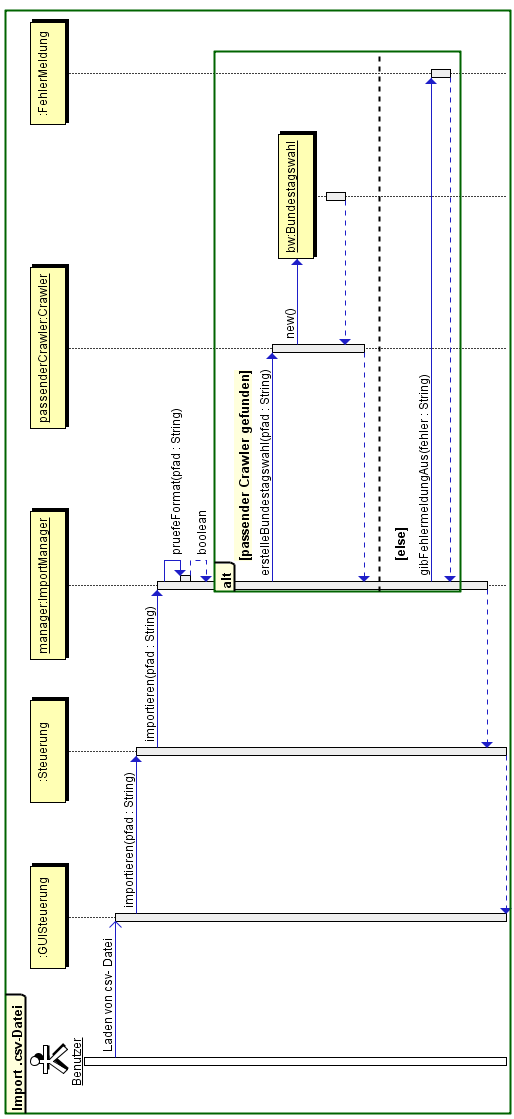
\includegraphics[scale=0.7]{Import-Sequenzdiagramm.png} 

\subsection{Export}
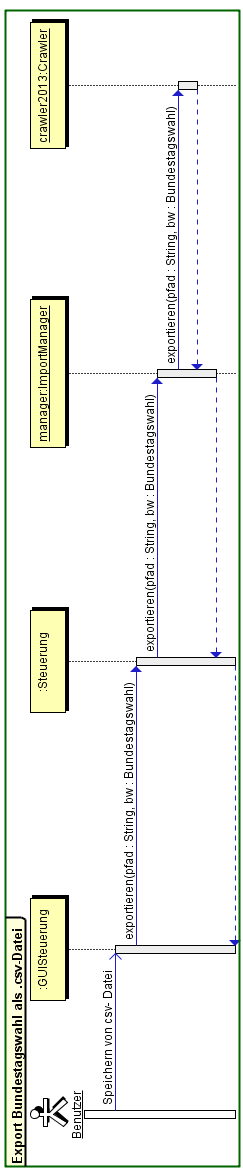
\includegraphics[scale=0.75]{Export-Sequenzdiagramm.png} 

\subsection{Paradoxe Wahlgenerierung und Vergleich}
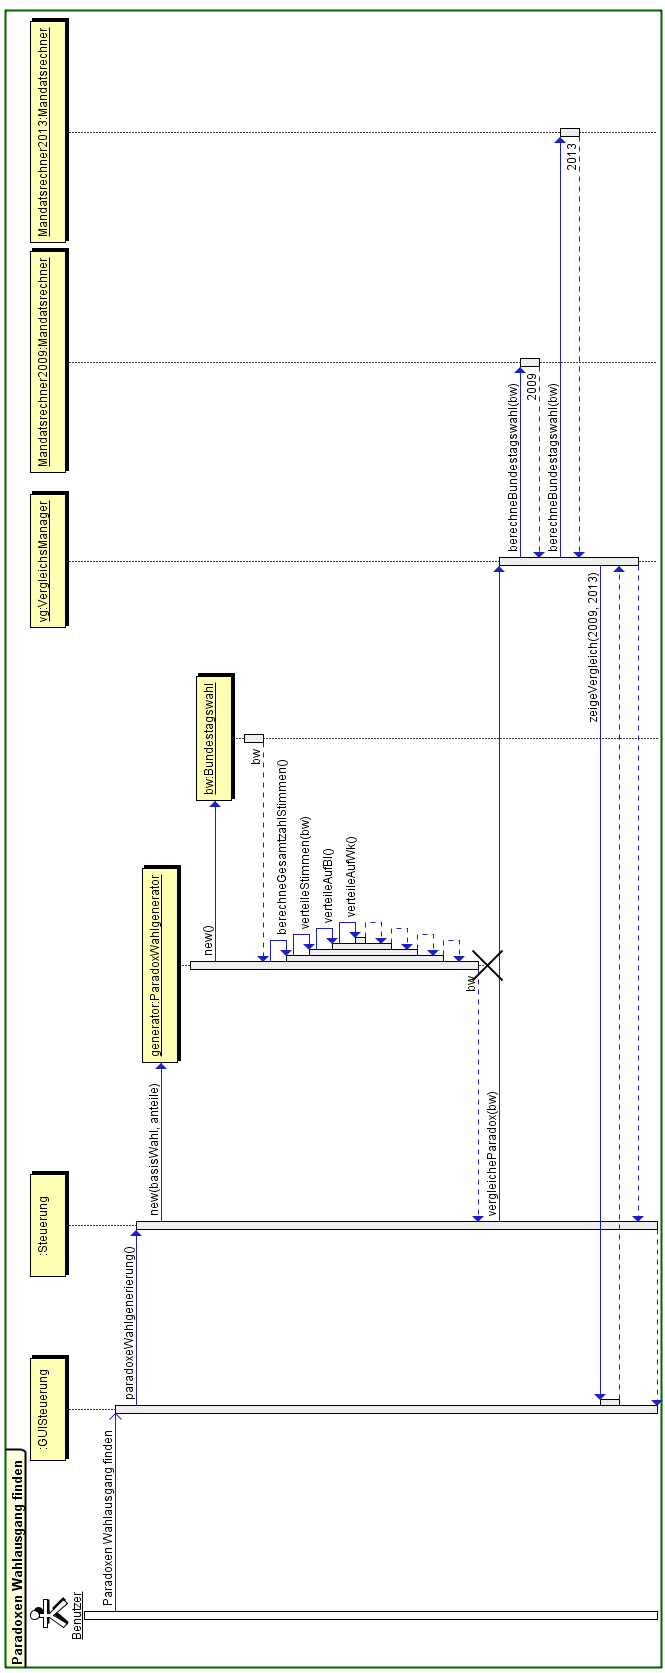
\includegraphics[scale=0.75]{paradoxeWahlgenerierung+Vergleich-Sequenzdiagramm.png} 

\subsection{Vergleich}
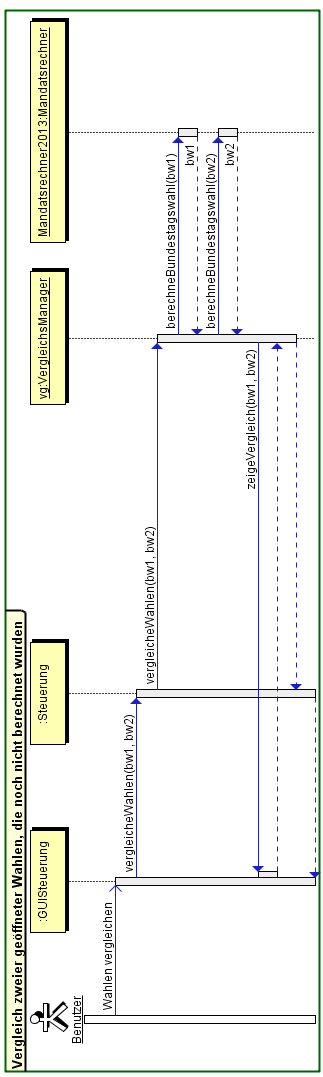
\includegraphics[scale=0.75]{Vergleich-Sequenzdiagramm.png} 

In diesem Sequenzdiagramm wird gezeigt, was passiert, wenn der Benutzer zwei Tabs geöffnet hat und einen Vergleich starten will.

\begingroup
\parindent 0pt
\parskip 2ex
\def\enotesize{\normalsize}

\endgroup
\end{document}
